\documentclass[cs4size,a4paper]{ctexart}   
%==================== 数学符号公式 ============
\usepackage{amsmath}                 % AMS LaTeX宏包
\usepackage[style=1]{mdframed}
\usepackage{amsthm}
\usepackage{pdfpages}
\usepackage{amsfonts}
\usepackage{mathrsfs}                % 英文花体字 体
\usepackage{bm}                      % 数学公式中的黑斜体
\usepackage{manfnt}           % 一些图标,如 \dbend
\usepackage{lettrine}                % 首字下沉,命令\lettrine
\def\attention{\lettrine[lines=2,lraise=0,nindent=0em]{\large\textdbend\hspace{1mm}}{}}
\usepackage{longtable}
\usepackage[toc,page]{appendix}
\usepackage{geometry}                % 页边距调整
\geometry{top=3.0cm,bottom=2.7cm,left=2.5cm,right=2.5cm}
%====================公式按章编号==========================
\numberwithin{equation}{section}
\numberwithin{table}{section}
\numberwithin{figure}{section}
%================= 基本格式预置 ===========================
\usepackage{fancyhdr}
\pagestyle{fancy}
\fancyhf{}  
\fancyhead[C]{\zihao{5}  \kaishu 这是一份实验报告}
\fancyfoot[C]{~\zihao{5} \thepage~}
\renewcommand{\headrulewidth}{0.65pt} 
\CTEXsetup[format={\centering\bfseries\zihao{-2}},name={第, 章}]{section}
\CTEXsetup[nameformat={\bfseries\zihao{3}}]{subsection}
\CTEXsetup[nameformat={\bfseries\zihao{4}}]{subsubsection}

%================== 表格 =========================
\usepackage{makecell,rotating,multirow,diagbox}
%================== 图形支持宏包 =========================
\usepackage{subfigure}
\usepackage{graphicx}                % 嵌入png图像
\usepackage{color,xcolor}            % 支持彩色文本、底色、文本框等
\usepackage{hyperref}                % 交叉引用
%\usepackage{caption}
\usepackage[font=small,labelfont=bf,labelsep=space]{caption}
\captionsetup{figurewithin=section}
%==================== 源码和流程图 =====================
\usepackage{listings}                % 粘贴源代码
\usepackage{xcolor}
\usepackage{color}
\definecolor{dkgreen}{rgb}{0,0.6,0}
\definecolor{gray}{rgb}{0.5,0.5,0.5}
\definecolor{mauve}{rgb}{0.58,0,0.82}
\usepackage{xcolor}

\definecolor{dkgreen}{rgb}{0,0.6,0}
\definecolor{gray}{rgb}{0.5,0.5,0.5}
\definecolor{comment}{rgb}{0.56,0.64,0.68}
\lstset{
  frame=tb,
  aboveskip=3mm,
  belowskip=3mm,
  xleftmargin=2em,
  xrightmargin=2em,
  showstringspaces=false,
  keepspaces=true,
 columns=flexible,
  framerule=1pt,
  rulecolor=\color{gray!35},
  backgroundcolor=\color{gray!5},
  basicstyle={\small\ttfamily},
  numbers=none,
  numberstyle=\tiny\color{gray},
  keywordstyle=\color{blue},
  commentstyle=\color{comment},
  stringstyle=\color{dkgreen},
  breaklines=true,
  breakatwhitespace=true,
  tabsize=2,
}
% \lstset{
% breaklines=true,
%  %行号
%    numbers=left,
%     numberstyle= \tiny, 
%    basicstyle=\tiny,
%    %背景框
%    framexleftmargin=8mm,
%    frame=none,
%     %背景色
%    %backgroundcolor=\color[rgb]{1,1,0.76},
%     backgroundcolor=\color[RGB]{245,245,244},
%     %样式
%   keywordstyle=\bf\color{blue},
%   identifierstyle=\bf,
%    numberstyle=\color[RGB]{0,192,192},
%    commentstyle=\it\color[RGB]{0,96,96},
%   stringstyle=\rmfamily\slshape\color[RGB]{128,0,0},
%   %显示空格
%    showstringspaces=false
% }


%--------------------
\hypersetup{hidelinks}
\usepackage{booktabs}  
\usepackage{shorttoc}
\usepackage{tabu,tikz}
\usepackage{float}

\usepackage{multirow}



\tabcolsep=1ex
\tabulinesep=\tabcolsep
\newlength\tikzboxwidth
\newlength\tikzboxheight
\newcommand\tikzbox[1]{%
        \settowidth\tikzboxwidth{#1}%
        \settoheight\tikzboxheight{#1}%
        \begin{tikzpicture}
        \path[use as bounding box]
                (-0.5\tikzboxwidth,-0.5\tikzboxheight)rectangle
                (0.5\tikzboxwidth,0.5\tikzboxheight);
        \node[inner sep=\tabcolsep+0.5\arrayrulewidth,line width=0.5mm,draw=black]
                at(0,0){#1};
        \end{tikzpicture}%
        }

\makeatletter
\def\hlinew#1{%
  \noalign{\ifnum0=`}\fi\hrule \@height #1 \futurelet
   \reserved@a\@xhline}
   
\newcommand{\tabincell}[2]{\begin{tabular}{@{}#1@{}}#2\end{tabular}}%

\usepackage{subfigure}

\usepackage{CJK}
\usepackage{ifthen}


\usepackage{graphicx} 
\newcommand{\HRule}{\rule{\linewidth}{0.5mm}}

\newtheorem{Theorem}{定理}
\newtheorem{Lemma}{引理} 
%%使得公式随章节自动编号
\makeatletter
\@addtoreset{equation}{section}
\makeatother
\renewcommand{\theequation}{\arabic{section}.\arabic{equation}}

%-------------------------
	
\usepackage{pythonhighlight}
\usepackage{tikz}                    
\usepackage{tikz-3dplot}
\usetikzlibrary{shapes,arrows,positioning}
%===================   正文开始    ===================
\begin{document}
\bibliographystyle{gbt7714-2005}     %论文引用格式
%===================  定理类环境定义 ===================
\newtheorem{example}{例}              % 整体编号
\newtheorem{algorithm}{算法}
\newtheorem{theorem}{定理}            % 按 section 编号
\newtheorem{definition}{定义}
\newtheorem{axiom}{公理}
\newtheorem{property}{性质}
\newtheorem{proposition}{命题}
\newtheorem{lemma}{引理}
\newtheorem{corollary}{推论}
\newtheorem{remark}{注解}
\newtheorem{condition}{条件}
\newtheorem{conclusion}{结论}
\newtheorem{assumption}{假设}
%==================重定义 ===================
\renewcommand{\contentsname}{目录}     
\renewcommand{\abstractname}{摘要} 
\renewcommand{\refname}{参考文献}     
\renewcommand{\indexname}{索引}
\renewcommand{\figurename}{图}
\renewcommand{\tablename}{表}
\renewcommand{\appendixname}{附录}
\renewcommand{\proofname}{证明}
\renewcommand{\algorithm}{算法} 
%============== 封皮和前言 =================
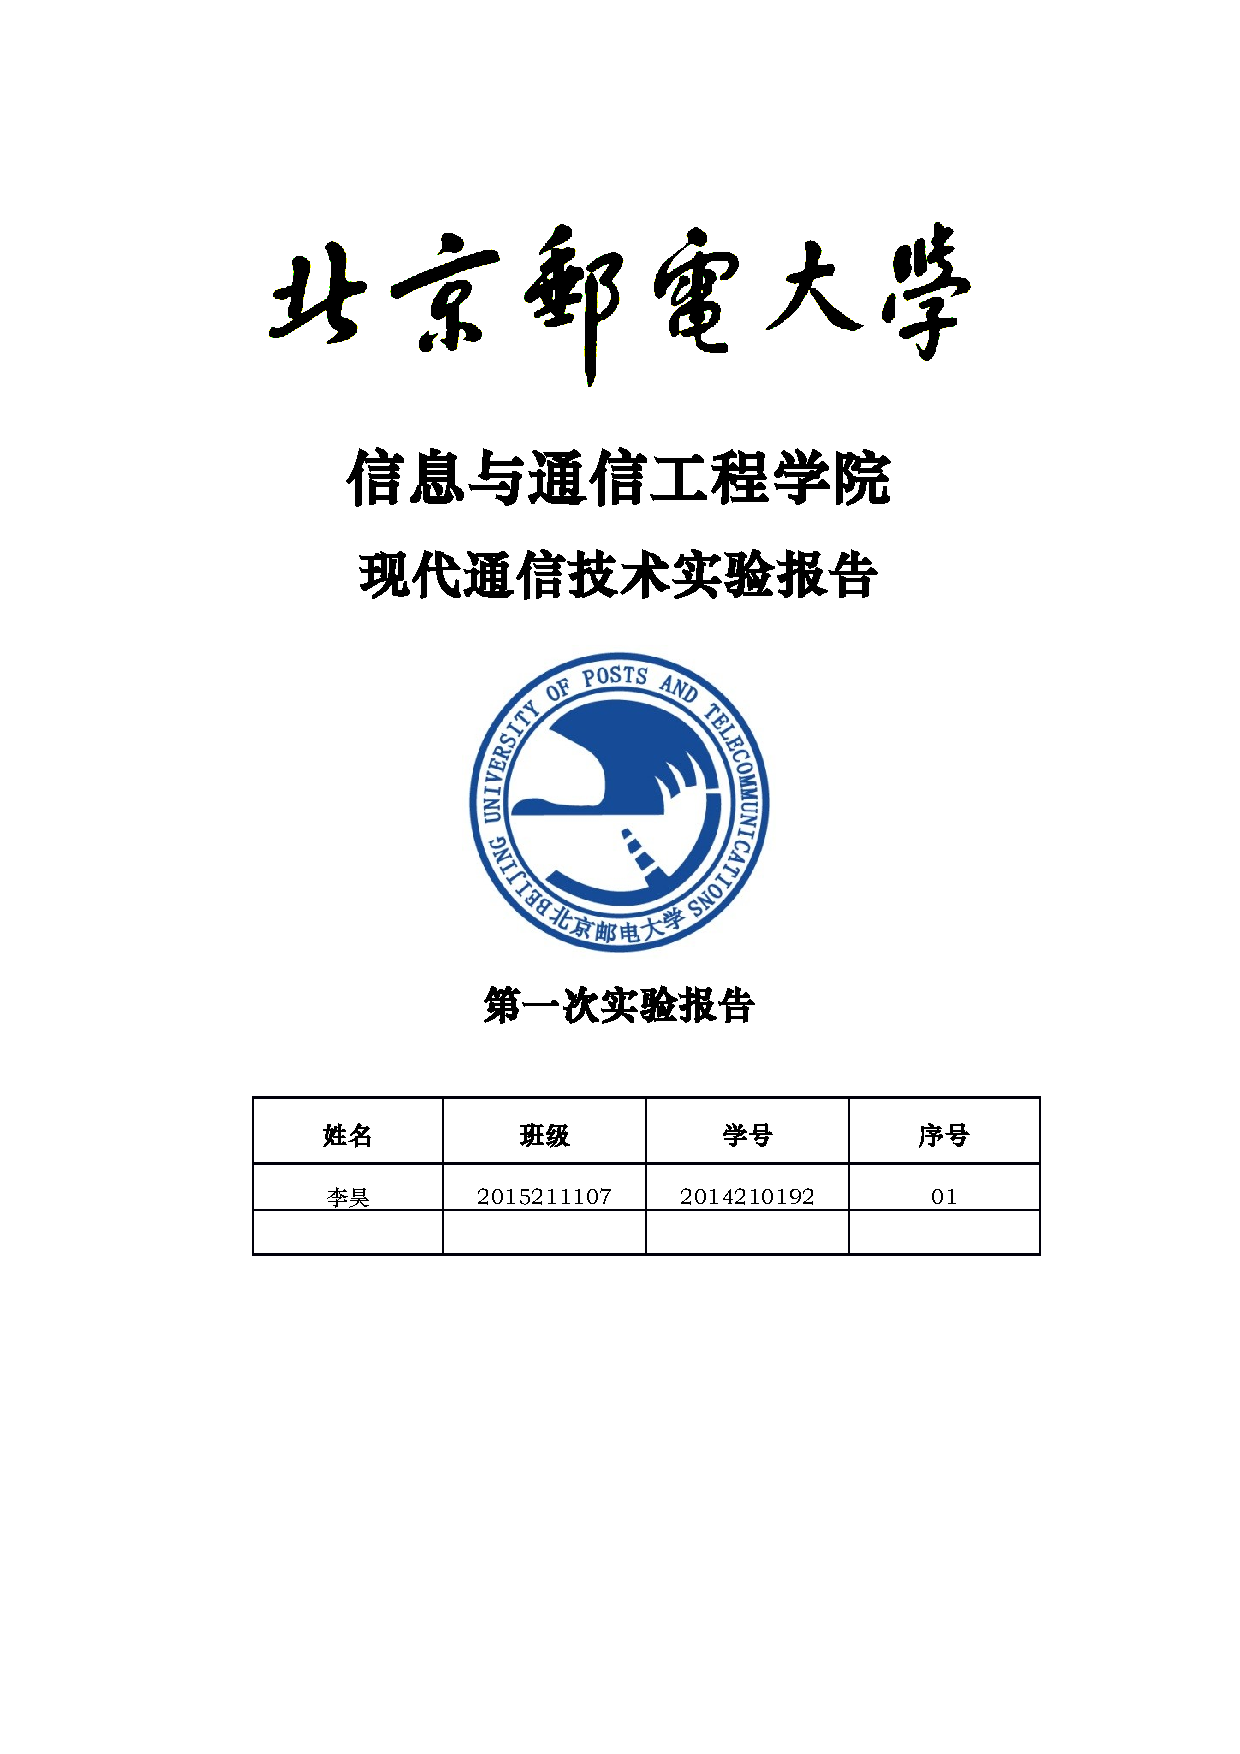
\includepdf[page=1]{cover/cover}
\pagestyle{plain}
\pagenumbering{roman}
\section*{\zihao{3} \centering 摘要}

\vskip0.5cm
本设计旨在用最少的设备去模拟一个校园网的网络环境.在连接功能上能够实现内部所有终端能够访问外网,服务器对内网和外网均开放.安全方面实现不同部门之间隔离但是内部互通, 教学区和非教学区隔离.ip分配上实现服务器用静态ip分配, 其他终端用动态ip分配.服务器内容方面有校园网站,文件共享,内网dns三个服务.

\textbf{关键词:}  校园网 ACL,VLAN,DHCP,NAY, DNS
\addcontentsline{toc}{section}{摘要}

\clearpage
\section*{\zihao{2} \centering \textbf{Abstract} }
   %用了Times New Roman字体来美化观感
Our design aimed at simulating the network environment of a campus network with a minimum number of equipments.
On the point of connection function,all of our inside hosts can visit the Internet.What'more,the server is open to
both the intranet and the outer network.In terms of security ,what we have already relized is the isolation between
different departments but interoperability,isolation of teaching and non teaching areas.AS  for IP allocation,
the server is allocated in a static IP, and the other terminals are allocated with dynamic IP.Also,there are three services:campus web site,file sharing and internal network DNS.  

\textbf{Key Words:}Campus network ,ACL ,VLAN ,DHCP ,NAT ,DNS 
\addcontentsline{toc}{section}{Abstract}





%\pagestyle{empty}
\tableofcontents 
%\thispagestyle{empty}
%============== 论文正文   =================
\pagestyle{fancy}
\pagenumbering{arabic}

\section{示例}

\subsection{插入图片}
如图\ref{fig:logo}所示,这是一个滑稽\\
%插入图片[图片宽度/页宽]{path}{label}{caption}
\addfig[0.2]{logo.jpg}{fig:logo}{滑稽的基类}

\subsection{插入代码}
\addcode[python]{code.py}

\subsection{插入数学公式}
%https://zh.numberempire.com/latexequationeditor.php, 在这个网站上生成公式代码
$$ \frac{\partial f}{\partial x} = 2\,\sqrt{a}\,x $$

\subsection{插入表格}
如\ref{table}所示, 这是一个表格
\begin{table}[H]
 \centering 
\begin{tabular}{|c|*{4}{c}|}
\hline
\diagbox{序号1}{序号2} & A & B & C& D \\
\hline
数字 & 1 & 2 & 3 & 4 \\
\hline
数字 & 2 & 4 & 6 & 8 \\
\hline
\end{tabular}
\caption{表格}\label{table}  
\end{table}


\subsection{关于缩进}
\indent \textbf{xxxx}\\
\noindent xxxx

\subsection{list}
\begin{enumerate}
	\item  啊啊啊啊啊
	\item  嗯嗯嗯嗯恩???
\end{enumerate}
\begin{description}
  \item[牛逼的人] linus, stallman 
  \item[牛逼的工具] git, gnuplot
\end{description}
\begin{itemize}
	\item A
	\item B
\end{itemize}
      %
%\pagenumbering{arabic}

\section{示例}

\subsection{插入图片}
如图\ref{fig:top_realmeaning}所示\\
\begin{figure}[thbp!]
\centering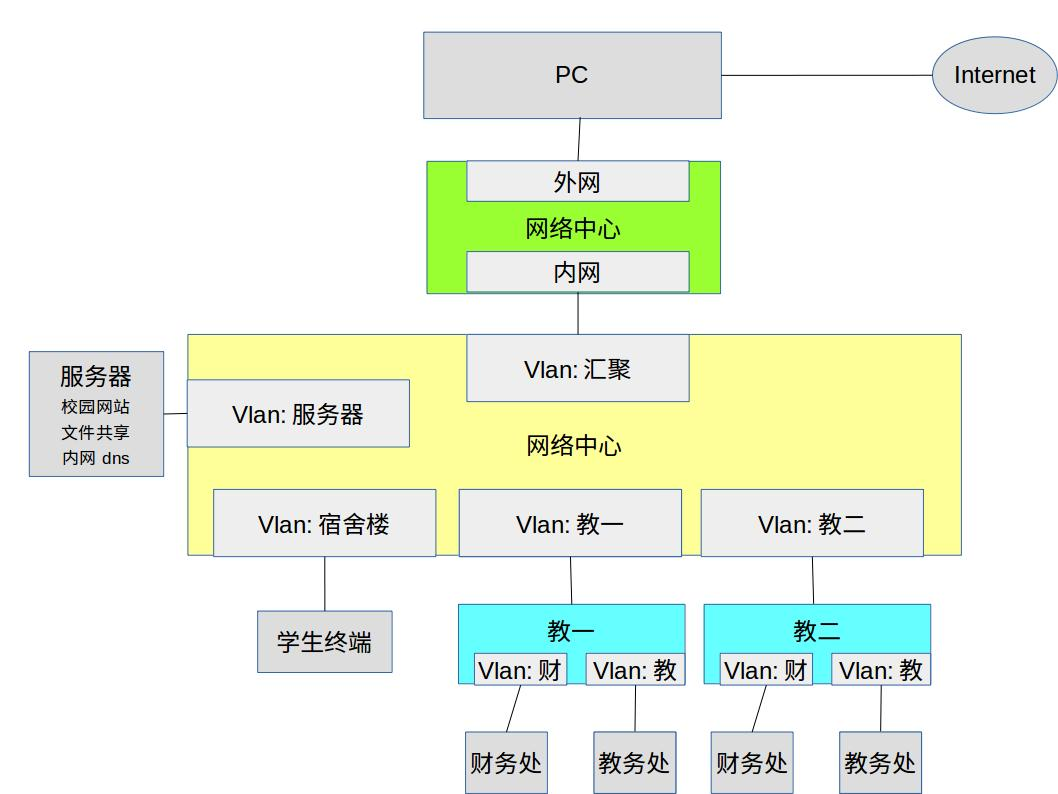
\includegraphics[width=0.9\linewidth]{figure/top_realmeaning.jpg}
\caption{ 模拟场景}
\label{fig:top_realmeaning}
\end{figure}

\subsection{插入代码}
\begin{lstlisting}[language=matlab]
  a=a;
  b=b;
  c=xxx;
\end{lstlisting}

\subsection{插入表格}
\begin{tabular}{cc}%一个c表示有一列,格式为居中显示(center)
(1,1)&(1,2)\\%第一行第一列和第二列  中间用&连接
(2,1)&(2,2)\\%第二行第一列和第二列  中间用&连接
\end{tabular}

\subsection{关于缩进}
\indent \textbf{xxxx}\\
\noindent xxxx

\subsection{list}
\begin{enumerate}
	\item A
	\item B
	\item C
\end{enumerate}

      %
%============= 参考文献 =====================
\addcontentsline{toc}{section}{参考文献}
\begin{thebibliography}{9}
\bibitem{latexcompanion} 
魏楚原 等.《大型园区网络建设与管理》.机械工业出版社.2015.3 
\bibitem{einstein} 
乔辉,刘晓辉,张新明 等.《网络硬件搭建与配置实践》.第三版.电子工业出版社.2012.5:第三章第二节
\bibitem{knuthwebsite} 



杜洪乐.《计算机网络实验指导书》.天津大学出版社.2016.3:
\end{thebibliography}
\clearpage

%=============  致谢  ======================
%\section*{致谢}
\addcontentsline{toc}{section}{致谢}
感谢父母为我提供的良好的衣食条件,让我有精力投入到这项没有经济回报的项目中去。
感谢徐海祥老师为我定制的论文题目,这个题目让我有兴趣制作这个模板。感谢武汉理工大学博士与硕士论文作者Hu,Weiyi,我在本模板制作的过程中参考了前辈的思路的方法。我研究过的模板还包括:上海交通大学,清华大学,哈尔滨工业大学,以及中国科技大学。其中论文引用格式GBT7714-2005-BibTeX-Style是上海财经大学的Haixing Hu作品,本模板离不开这些有益的资源的支持。同样感谢正在使用这个模板的你,相信通过你们的使用和传播,这个模板会变得越来越完善。
%\newpage
\appendix

%%附录第一个章节
\section{第一附录}


%%变量列举

\begin{table}[H]
\caption{Symbol Table-Constants}
\centering
\begin{tabular}{lll}
\toprule
Symbol & Definition  & Units\\
\midrule[2pt]
\multicolumn{3}{c}{\textbf{Constants} }\\
$DL$&Expectancy of poisson-distribution &  unitless \\
$NCL$ &Never- Change-Lane& unitless\\
$CCL$&Cooperative-Change-Lane& unitless\\
$ACL$&Aggressive-Change-Lane& unitless\\
$FCL$&Friendly-Change-Lane& unitless\\
$SCC$&Self-driving-Cooperative-Car& unitless\\
$NSC$&None-Self-drive-Car& unitless\\
\bottomrule
\end{tabular}
\end{table}


\section{第二附录}
\textcolor[rgb]{0.98,0.00,0.00}{\textbf{Simulation Code}}
\begin{python}
import java.util.*;  
public class test {  
    public static void main (String[]args){   
        int day=0;  
        int month=0;  
        int year=0;  
        int sum=0;  
        int leap;     
        System.out.print("请输入年,月,日\n");     
        Scanner input = new Scanner(System.in);  
        year=input.nextInt();  
        month=input.nextInt();  
        day=input.nextInt();  
        switch(month) /*先计算某月以前月份的总天数*/    
        {     
        case 1:  
            sum=0;break;     
        case 2:  
            sum=31;break;     
        case 3:  
            sum=59;break;     
        case 4:  
            sum=90;break;     
        case 5:  
            sum=120;break;     
        case 6:  
            sum=151;break;     
        case 7:  
            sum=181;break;     
        case 8:  
            sum=212;break;     
        case 9:  
            sum=243;break;     
        case 10:  
            sum=273;break;     
        case 11:  
            sum=304;break;     
        case 12:  
            sum=334;break;     
        default:  
            System.out.println("data error");break;  
        }     
        sum=sum+day; /*再加上某天的天数*/    
        if(year%400==0||(year%4==0&&year%100!=0))/*判断是不是闰年*/    
            leap=1;     
        else    
            leap=0;     
        if(leap==1 && month>2)/*如果是闰年且月份大于2,总天数应该加一天*/    
            sum++;     
        System.out.println("It is the the day:"+sum);  
        }  
} 
\end{python}



%============= 工作日志  ===================
%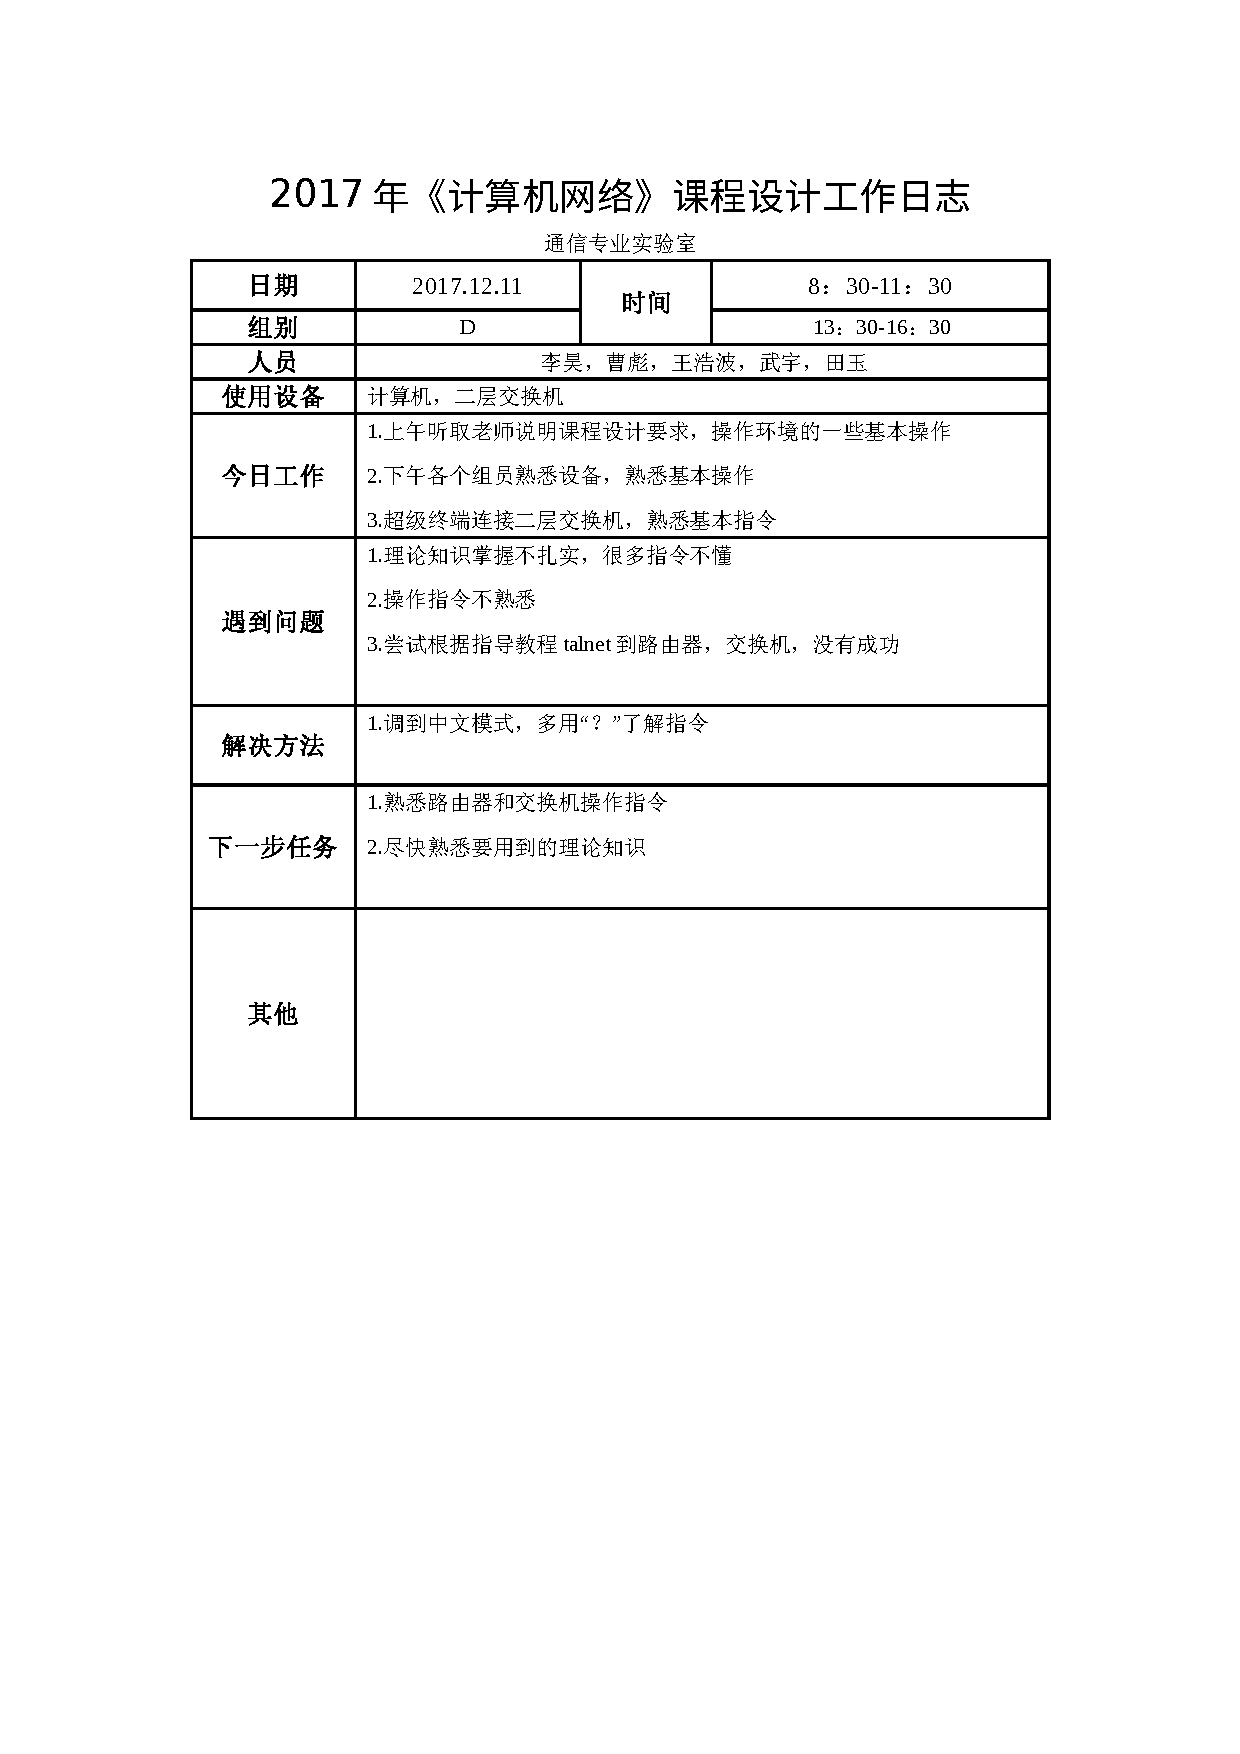
\includepdf[pages=1-10]{body/log}

\end{document}
%%%%%%%%%% 结束 %%%%%%%%%%
